%%%%%%%%%%%%%%%%%%%%%%%%%%%%%%%%%%%%%%%%%%%%%%%%%
%%%%%%%%%%%%%%%%%%%%%%%%%%%%%%%%%%%%%%%%%%%%%%%%%

\chapter{Experimental Setup}
\label{chap:third}

%%%%%%%%%%%%%%%%%%%%%%%%%%%%%%%%%%%%%%%%%%%%%%%%%
%%%%%%%%%%%%%%%%%%%%%%%%%%%%%%%%%%%%%%%%%%%%%%%%%

This chapter details the experimental setup for the simulations that were performed. The parameters used in the experiment are explained in Section~\ref{parameters}, while Section~\ref{thri:third:performancemeasures} defines the performance measures used to evaluate the results of the experiment. Finally, section~\ref{thri:third:environmenttypes} discusses the environment types and how they have been generated, and the process is summarized in Section~\ref{third:summary}

%%%%%%%%%%%%%%%%%%%%%%%%%%%%%%%%%%%%%%%%%%%%%%%%%
%%%%%%%%%%%%%%%%%%%%%%%%%%%%%%%%%%%%%%%%%%%%%%%%%

%Parameter
\section{Parameters}
\label{parameters}

For each class of environment, the following configurations were tested: The environment grid size, $S=50,100,200,300, 500$ where $S$ is the width and length of the grid and the percentage of the grid covered by items $p$, where $p= 0.05\%$, $0.2\%$, $0.5\%$, $0.7\%$, $0.9\%$. The ratio of prioritized to non-prioritized items $r$, is varied, where $r=0$, $0.2$,$0.25$, $0.333$, $0.5$, $0.667$, $0.75$, $0.8$, $1$. Honey bee specific parameters were selected based on \cite{seeley2009wisdom} as 
$t_{max}=200$ time steps, $f_{max}=100$ time steps, $\phi=0.8$ and $\rho=0.1$.

For all algorithms, robots were initially configured to forage either the prioritized item or the non-prioritized item with a ratio of $\tau=0$, $0.2$, $0.25$, $0.333$, $0.5$, $0.667$, $0.75$, $0.8$,$1$. The density of robots, $c$, is defined as the percentage of cells of the grid size $S$ (the length of the side of an environment) that are occupied by robots, where $c=0.1, 0.3, 0.5, 0.7, 1$.

All agents begin at random positions adjacent to the sink in the exploration state. All algorithms were run for 10000 time steps, where an agent can move maximum 1 grid cell at a time, to any adjacent cell not occupied by another robot or item. For all algorithms, the agents begin randomly positioned next to the sink. The beacon locating of the sinks is simulated by each agent evaluating and moving up a light intensity gradient. The colour of the light is used to distinguish between the 2 sinks.

\section{Performance Measures}
\label{thri:third:performancemeasures}

%What do I need to add to 
%TODO: The idea is to add more robots foraging the prioritized items.
The following performance measures were used: 

	\begin{itemize}
		\item	The percentage of prioritized items foraged over time,  $\sigma$ 
		\item	The percentage of non-prioritized items foraged over time, $\mu$
		\item   The average time spent by agents waiting at the sink, $\epsilon$
	\end{itemize}
	
Future studies could include the average time taken by a robot to forage an item, the average distance moved by a robot and a measure to explain the randomness of a robots movement. 
%%%%%%%%%%%%%%%%%%%%%%%%%%%%%%%%%%%%%%%%%%%%%%%%%

\section{Environment Types}
\label{thri:third:environmenttypes}
Each environment type was chosen to examine specific capabilities of the algorithms. Four different classes of environments were randomly generated as follows:
\begin{enumerate}
\item Environments where items of each type are uniformly distributed (Fig \ref{fig:uniformenv}). The uniformly distributed environment is used as a base line to test the algorithms.
\item Clustered environments have clusters of item types generated by randomly relabelling the items in clusters that are generated by Lumer-Faieta ant cemetery clustering \cite{lumer1994diversity} as either prioritized or non-prioritized items (Fig \ref{fig:clusterenv}). These algorithms test the algorithms ability to exploit item rich areas. It will also test how effectively an agent can navigate around non-prioritized items. 
\item Vein environments resemble the patterns observed in naturally occurring gold \cite{frimmel2002recent} (Fig \ref{fig:veinenv}). The vein environments will test whether an agents of a specific algorithm can take advantage of the tunnel created by foraging items in the vein. 
\item Gaussian environments have prioritized items focused around the environment center in a gaussian distribution and the non-prioritized item conversely placed in the inverse distribution. (Fig \ref{fig:gaussianenv}). The gaussian environments are used to specifically examine how an algorithm can deal with moving past non-prioritized items to reach prioritized items. 
\end{enumerate} 

\vspace{-2em}
\begin{figure} [h]
        \centering
        \begin{subfigure}[b]{0.21\textwidth}
                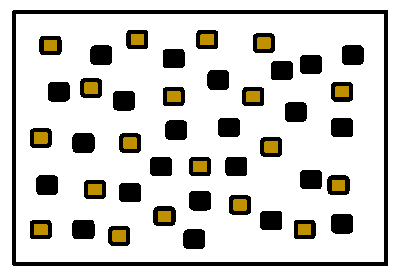
\includegraphics[width=\textwidth]{chapters/chapter4/figures/uniformenv.pdf}
                \caption{Uniform}
                \label{fig:uniformenv}
        \end{subfigure}%
        \begin{subfigure}[b]{0.205\textwidth}
                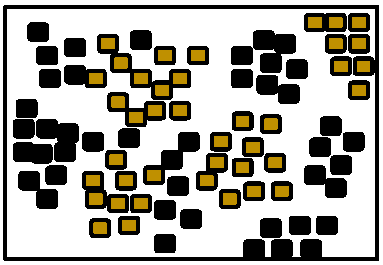
\includegraphics[width=\textwidth]{chapters/chapter4/figures/clusterenv.pdf}
                \caption{Clustered}
                \label{fig:clusterenv}
        \end{subfigure}
        \begin{subfigure}[b]{0.2\textwidth}
                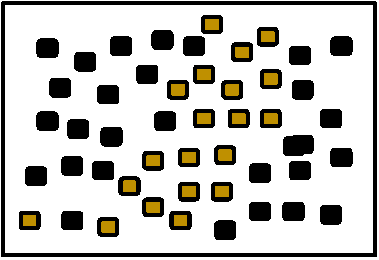
\includegraphics[width=\textwidth]{chapters/chapter4/figures/veinenv.pdf}
                \caption{Vein}
                \label{fig:veinenv}
        \end{subfigure}  
        \begin{subfigure}[b]{0.2\textwidth}
                        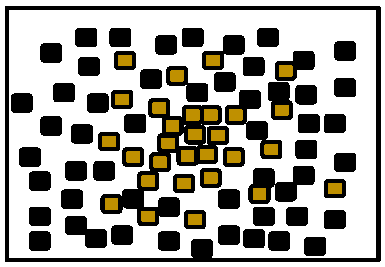
\includegraphics[width=\textwidth]{chapters/chapter4/figures/gaussianenv}
                        \caption{Gaussian}
                        \label{fig:gaussianenv}
       \end{subfigure}
        \caption{Environment Classes}\label{fig:environments}
\end{figure}


%%%%%%%%%%%%%%%%%%%%%%%%%%%%%%%%%%%%%%%%%%%%%%%%%
%%%%%%%%%%%%%%%%%%%%%%%%%%%%%%%%%%%%%%%%%%%%%%%%%
\section{Summary}
\label{third:summary}

This section details the parameters chosen for the algorithms as well as the performance measures selected in order to compare various aspects of the algorithms: the different percentages of each type of item foraged as well as the time spent waiting by the sink. Lastly, the environment types that were generated for experimentation in order to test different properties of the algorithms are discussed. The environment types defined have the four following distributions: uniform distribution, Gaussian distribution, clustered distribution and vein distribution. 


%%%
%%%%%%%%%%%%%%%%%%%%%%%%%%%%%%%%%%%%%%%%%%%%%%%%%
%%%%%%%%%%%%%%%%%%%%%%%%%%%%%%%%%%%%%%%%%%%%%%%%%